\chapter{AortaGeomRecon Research and Development}

This chapter will discuss the research and development of the 3D Slicer plugin AortaGeomRecon. AortaGeomRecon (AGR) stands for Aorta Geometry Reconstruction. The main objective of AGR is to semi-automatically build a 3D geometry of the aorta from the patient's chest CT scans.  The existing methods often involve extensive manual work interspersed with software assistance. An experienced user, who should be a medical domain expert, typically needs to do a minimum of 10 minutes of manual work. Currently, AGR allows users who have taken the university level anatomy introductory course to set the hyperparameters within half a minute, following by a maximum 2 minutes of execution time.

In this chapter, we first introduce the existing methods for aorta segmentation with different software options, and discuss the advantages and disadvantages of these existing options. Next, we demonstrate our segmentation algorithm, with a detailed step-by-step explanation of what the algorithm is doing and the results it generates. Finally, we discuss our experience using the platform 3D Slicer, and demonstrate our development results in the 3D Slicer plugin.

\section{Existing Methods}
There are many segmentation software options available to users. We will discuss two popular software options: \href{https://www.itksnap.org/}{ITK-Snap} and \href{https://www.slicer.org/}{3D Slicer}.

\subsection{ITK-Snap bubble method} 
ITK-Snap provides a segmentation method that first requires the user to select multiple voxels with a custom initial size and an expanding size within the volume. This method is referred to as the ``bubble method'' \cite{gerig}.

Through many iterations, the voxels expand to fill the entire volume of the vessel. As a final step, the user will need to cut off the extra parts of the volume. Figure~\ref{fig_ITK} shows ITK-Snap UI executing a segmentation of an aorta.

\begin{figure}[ht]
    \centering
    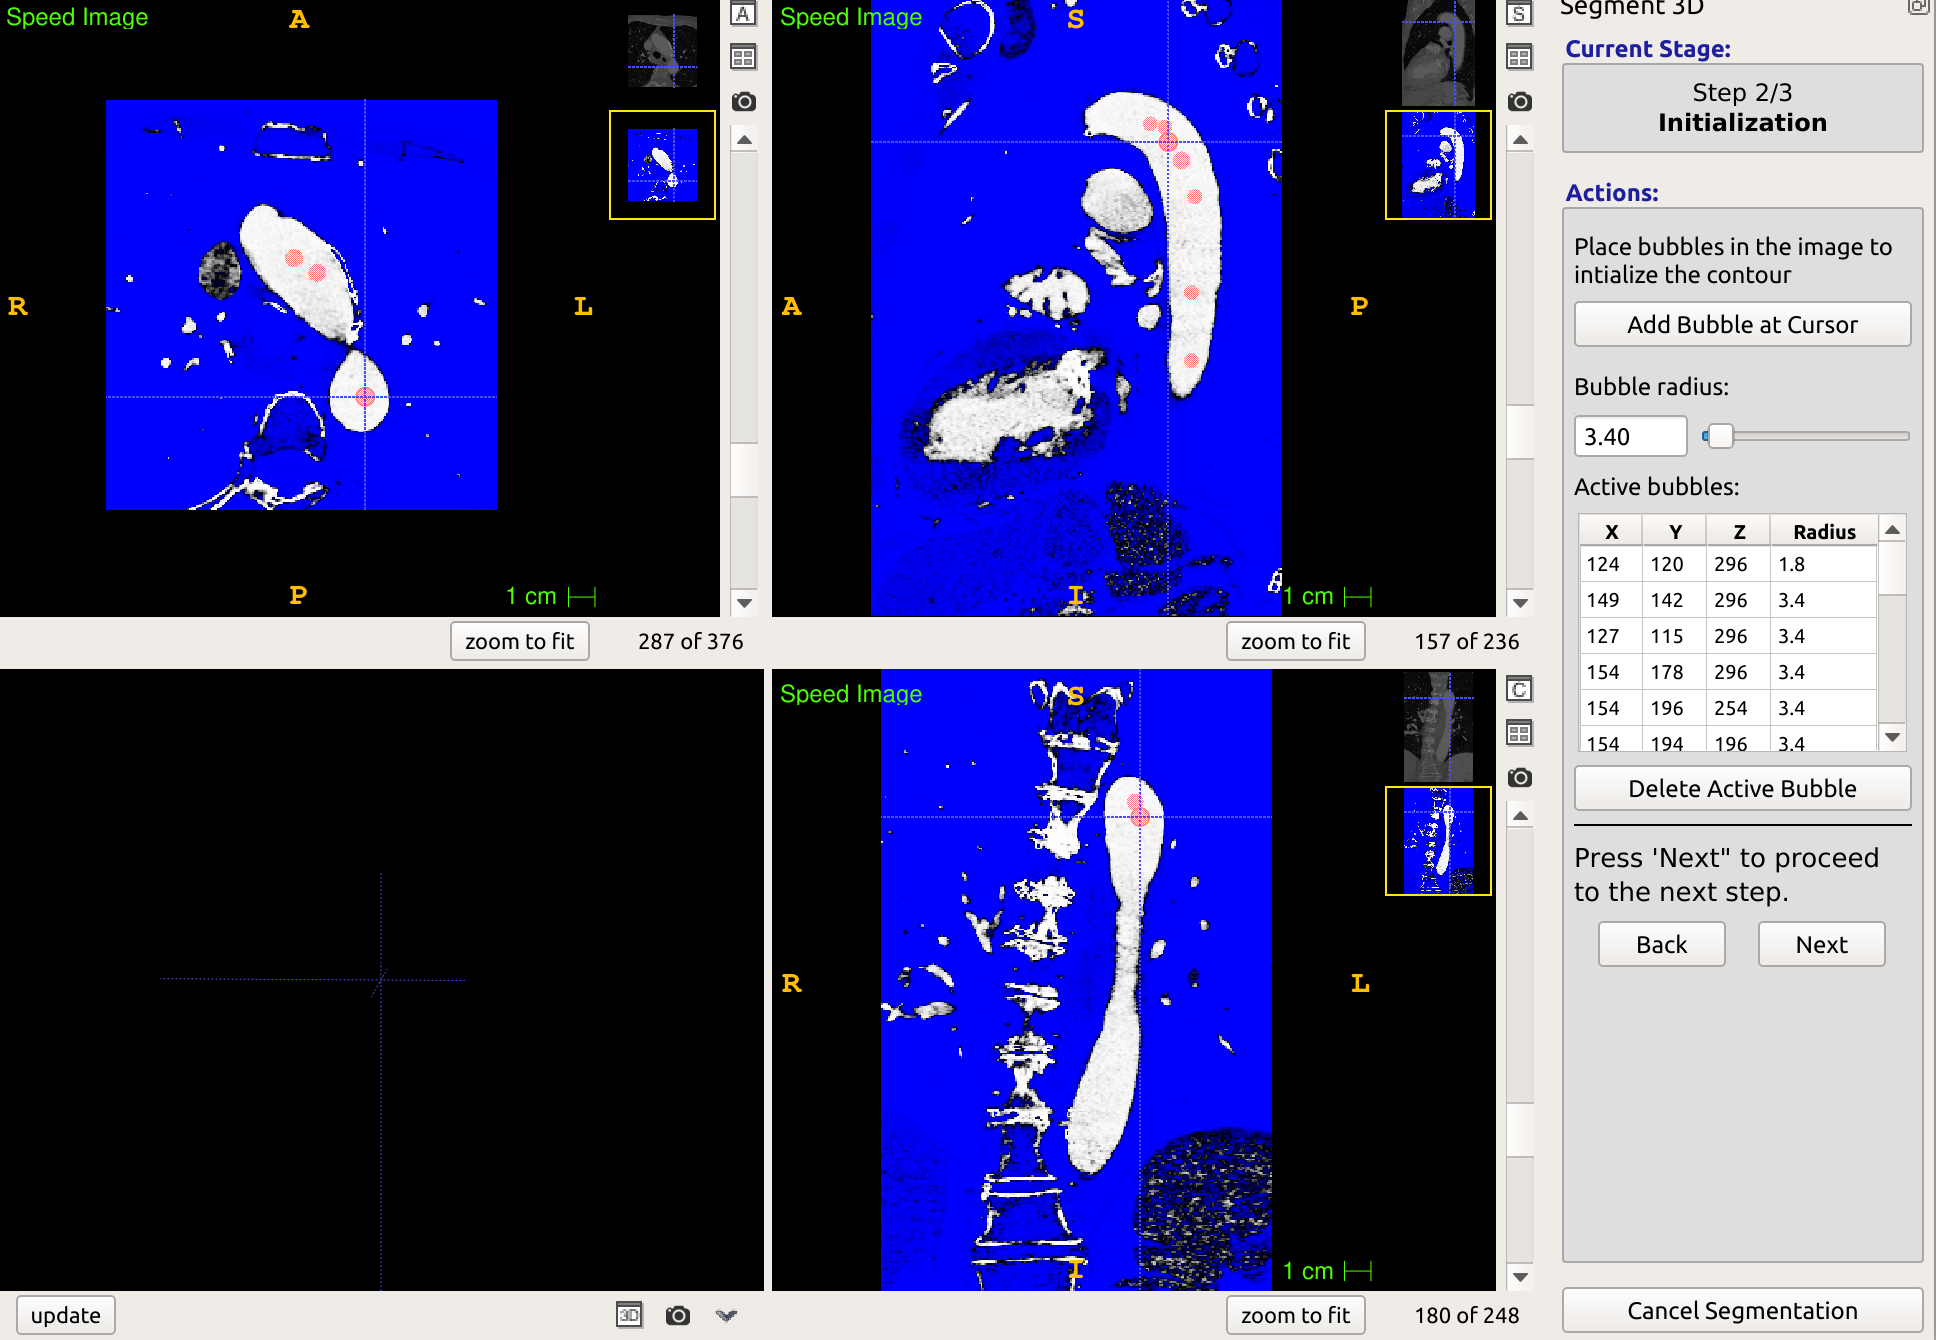
\includegraphics[width=0.8\textwidth]{figures/AGR/bubbles.png}
    \caption[ITK-Snap's Bubble Segmentation UI]{ITK-Snap's Bubble Segmentation UI \cite{py06nimg}}
    \label{fig_ITK}
\end{figure}

The advantage of the bubble method is that it is guaranteed to produce a correct segmentation for a valid image. A medical domain expert can manually control the desired area, and visually observe the segmentation result expanding, and shrinking. Moreover, the user can erase the unwanted parts.

The disadvantage of this method is that the operations described above are complicated. They are easier to say then do. An operator who has previous experience building the geometry with this method still needs about 20 minutes of manual work to build a new aorta geometry. Plus, ITK-Snap software can only read VTK (The Visualization Toolkit) files; therefore, the chest CT scans that are usually Digital Imaging and Communications in Medicine (DICOM) format \cite{10.1007/978-1-4020-8752-3_13}, needed a manual conversion step before using this software and its segmentation method.

\subsection{3D Slicer threshold segmentation}
3D Slicer is another well-known medical image processing software for academic uses. 3D Slicer provides multiple segmentation methods \cite{Slicer_Wiki}. One of the quickest and easiest to use is the intensity based segmentation.

This method first lets users select a small area that belongs to the wanted area on a 2D plane (Axial, Sagittal, and Coronal). 3D Slicer reads the pixel intensity of the surrounding area, and segments based on the intensity threshold. Any pixel's intensity that is within range will be segmented as the segmentation result, as demonstrated in Figure~\ref{fig_3D_Seg_Builtin}. 

The advantage of this method is that the user can visualize the effect of choosing different intensity threshold in real-time. 3D Slicer can highlight the pixels that would be chosen as a part of the segmentation with an increased or decreased intensity threshold.

The disadvantage of this method is that it depends on the quality of the input data. If the input data does not have the proper intensity reading of the aorta, it could generate gaps on the wanted part. Then, this method is less efficient, because the user must use another intensity range for the missing pixels. A \href{https://www.youtube.com/watch?v=5_673cHMBiY}{YouTube video} shows an experienced user who gets the aorta 3D geometry with 8 minutes of manual work. 

\begin{figure}[H]
    \centering
    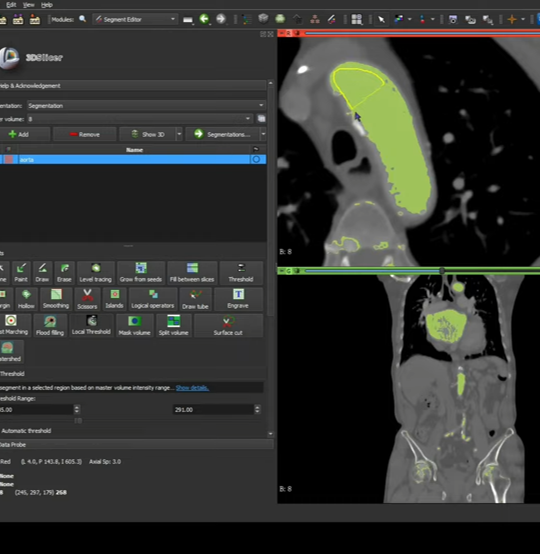
\includegraphics[width=0.7\textwidth]{figures/Sample/3D-Slicer-Segmentation.png}
    \caption[3D Slicer Built-in Segmentation UI]{3D Slicer Built-in Segmentation Method \cite{Kikinis2014}}
    \label{fig_3D_Seg_Builtin}
\end{figure}

\section{Our Segmentation Algorithm}

This section introduces the key concepts for the implementation of our segmentation algorithm. The algorithm is developed in Python with the external libraries SimpleITK and NumPy. The algorithm builds the 3D aorta geometry by doing segmentation on each axial slice. The logic behind segmenting each slice from the axial view is that there is one or two circles that are edge bounded in each axial plane view. Using this information, and given an initial aorta center coordinate, the algorithm continuously segments the axial slice's circles that are closest to the previous aorta center coordinates. Finally, some hyperparameters tuning can let the algorithm pick up the pixels that were missing but belongs to the aorta.

In this section, we first introduce the contexts for the external libraries used in the implementation of the algorithm. We show the parameters and hyperparameters of the algorithm. Then we explain the algorithm workflow with a step-by-step demonstration.

\subsection{Background} \label{algo_bg}

SimpleITK is an open-source multidimensional image analysis library developed by the Insight Toolkit community for the biomedical sciences and beyond \cite{JSSv086i08}\cite{10.3389/fninf.2013.00045}. NumPy is the fundamental package for scientific computing with Python, especially for the performance of multidimensional array processing \cite{harris2020array}. The algorithm will use functions from these two libraries for image processing and multidimensional array processing. For example, the algorithm segments each slice with ThresholdSegmentationLevelSetImageFilter from SITK.

The algorithm works best with the chest volume cropped to a rectangular prism that contains the aorta and parts of the other organs such as the backbone, blood vessels, and the heart. This can be done with 3D Slicer and its built-in modules, Volume rendering and Crop Volume, or researched by another means familiar to the user for finding the starting point and the size to crop.

\subsection{Parameters}

At the beginning of the algorithm, the user inputs two integer coordinates indicating the position of the descending aorta and ascending aorta center on a single slice. The yellow dots in Figure~\ref{fig_aorta_seed} shows an example of the aorta seeds. These seeds will be updated by the algorithm after processing each axial plane.

\begin{figure}[ht]
    \centering
    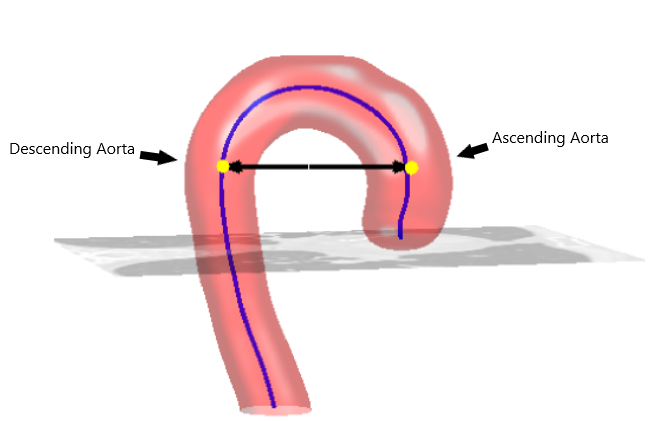
\includegraphics[width=0.7\textwidth]{figures/Sample/Aorta_seeds.png}
    \caption[The Aorta Seeds]{The aorta seeds \citep{6346433}}
    \label{fig_aorta_seed}
\end{figure}

The following list of hyperparameters that can be tuned to get the best segmentation result:
\begin{itemize}
\item The stop limit, which controls the stop condition
\item The threshold coefficient, which controls the segmentation acceptable intensity range
\item The kernel size, which controls the label image circle size 
\item The threshold Segmentation Level Sets Image Filter parameters, including:
\begin{itemize}
\item The RMS error
\item The maximum iteration
\item The curvature scaling
\item The propagation scaling
\end{itemize}
\end{itemize}

One of the most important parameters is the threshold coefficient. Since the algorithm segments based on the intensity of the gray scale pixels, decreasing the threshold coefficient decreases the acceptable range of the pixels, and vice-versa. 


\subsection{Algorithm Overview} \label{algo}

When the user has selected the aorta seeds, the plane where the aorta seeds are located is the initial plane. From this plane towards the bottom (toward the feet) is the inferior direction. The upward direction (toward the head) is the superior direction. This algorithm segments each slice with SITK::ThresholdSegmentationLevelSetImageFilter. The principles of this image filter can be explained with two terms: Level sets segmentation method, and a threshold range that defines the intensity of the acceptable pixel.

Level Sets are an important category of modern image segmentation techniques based on partial differential equations (PDE), i.e. progressive evaluation of the differences among neighboring pixels to find object boundaries. The pictures in Figure~\ref{LSS} demonstrate an example of how the Level Sets method work on finding the region of the heart. It starts with a seed contour that is within the region of interest, then by finding the gradient based on the contour line, the segmentation result will propagate towards the outside of the region, until the maximum difference between the neighboring pixels are reached.

\begin{figure}[H] 
\centering
\subfloat[\centering Init image]{{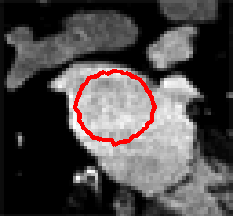
\includegraphics[width=0.33\textwidth]{figures/AGR/heart-1.png}}}%
\subfloat[\centering Expanding]{{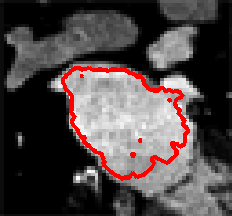
\includegraphics[width=0.33\textwidth]{figures/AGR/heart-2.png}}}%
\subfloat[\centering Result]{{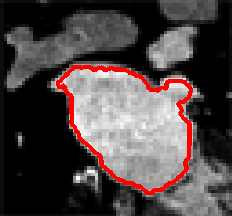
\includegraphics[width=0.33\textwidth]{figures/AGR/heart-3.png}}}%
\caption[Level Sets Segmentation]{Level Sets Segmentation}
\label{LSS}
\end{figure}

\subsection{The steps to segment a single slice}
In the following section, we will present each step to segment a single slice. These steps are applied for segmentations in both the superior and inferior directions. There is a difference in the stopping condition, which we will elaborate in Section~\ref{stopping_condition}.

\subsubsection{Create A Label Map}\label{label_map}
The algorithm uses SITK::BinaryDilateImageFilter to perform binary dilation to generate a circle-like shape around the center coordinates (user input’s for the first slice and calculated by the algorithm for the rest of the slices). The binary dilation helps to fill in and smooth out gaps where the image intensity drops. Each pixel within this shape will be labeled as a white pixel (value of 1), and the rest of the pixels are labeled as black pixels (value of 0). 

The generated result is the label map image. We will use it in the next few steps. The size of the circle-like shape is determined by the kernel size (user's input). The Figure \ref{fig_label_map} shows an example of generated label map image (the green parts) overlay over the original slice.

\begin{figure}[H]
    \centering
    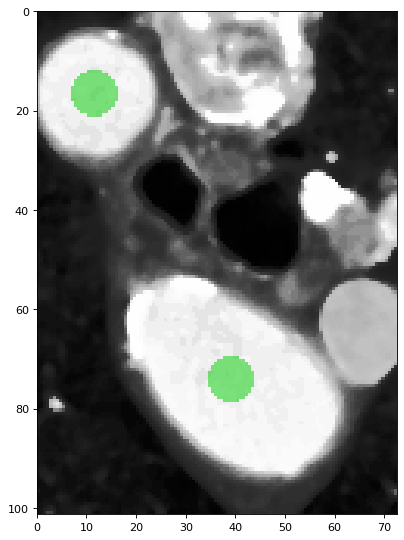
\includegraphics[width=0.4\textwidth]{figures/AGR/label_image.png}
    \caption[A label image]{A Label Map}
    \label{fig_label_map}
\end{figure}

\subsubsection{Create A Distance Map}\label{distance_map}
With SITK::SignedMaurerDistanceMapImageFilter, the algorithm creates another image, the Euclidean distance transform of the label image from previous step. This is used as a contour line that helps build the gradient mentioned in Level sets. The Figure \ref{fig_distance_map} shows an example of distance map.

\begin{figure}[H]
    \centering
    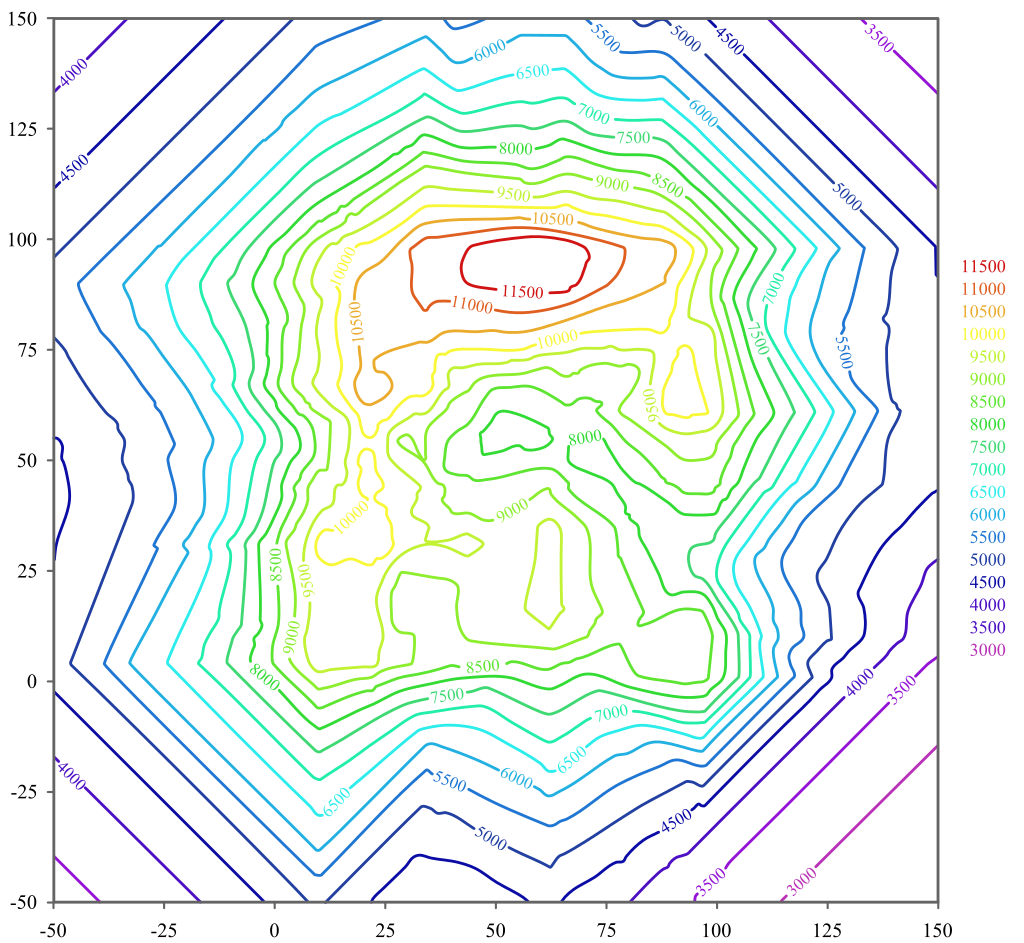
\includegraphics[width=0.45\textwidth]{figures/AGR/Contour2D.png}
    \caption[A Distance Map]{A Distance Map}
    \label{fig_distance_map}
\end{figure}

\subsubsection{Calculate A Threshold Range} \label{threshold}
By using SITK::LabelStatisticsImageFilter, the algorithm gets the mean and the standard deviation of the intensity values of the pixels that were labeled as the white pixel in the label map. The algorithm uses the threshold coefficient to calculate the lower and upper threshold to be used in the next step.

\begin{figure}[H]
    \centering
    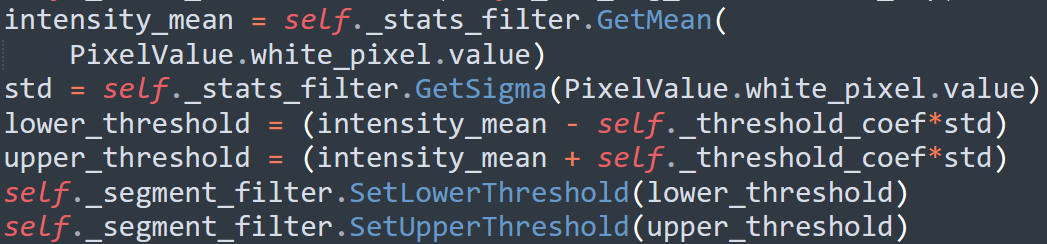
\includegraphics[width=0.7\textwidth]{figures/AGR/threshold.png}
    \caption[Code That Shows How To Calculate The Threshold Range]{Code That Shows How To Calculate The Threshold Range}
    \label{fig_threshold}
\end{figure}

\subsubsection{Segment A Single Slice}\label{segment}
With SITK::ThresholdSegmentationLevelSetImageFilter, the seed image calculated in step \ref{distance_map}, and the lower and upper threshold value calculated in step \ref{threshold}, the algorithm performs segmentation and generates a segmented slice. Figure~\ref{fig_segmented_image} shows an example of generated segmented slice (the green parts) overlay over the original slice.

\begin{figure}[H]
    \centering
    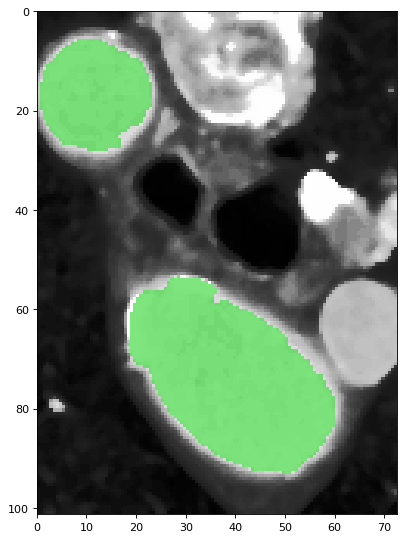
\includegraphics[width=0.5\textwidth]{figures/AGR/segment_label_image.png}
    \caption[A Segmented Image]{A Segmented Image On Top Of The Original Slice}
    \label{fig_segmented_image}
\end{figure}

\subsubsection{Calculate New Centroids}
By comparing each pixel segmented as aorta to the previous descending centroid and the previous ascending centroid, the algorithm use the positions of the points closer to the previous descending centroid to calculate the new descending aorta centroid, and vice-versa for the ascending aorta centroid. However, at a certain point during the segmentation in the inferior direction, the slice will reach the end of the ascending aorta, the aortic root. We will explain how we detect this scenario in section \ref{stopping_condition}. For the rest of the slices in the inferior direction, the algorithm will stop using, and calculating the ascending aorta centroid as it only requires the descending aorta centroid.

\subsubsection{Verify Segmentation Result}\label{stopping_condition}
There are two main stopping conditions for verifying segmentation result, one condition for the segmentation in the inferior direction and the other one for the segmentation in the superior direction. The stopping limit is a user defined parameter to control the algorithm, that would affect the result in this step.

In the inferior direction, if the new ascending aorta centroid that is closest to the previous ascending aorta center is reaching the distance limit, then the algorithm will stop and consider taking the new centroid closer to the ascending aorta. In other words, only one centroid will be used for the descending aorta segmentation.

In the superior direction, if the standard deviation of the initial label map and the segmentation result label map have larger differences than the limit, the algorithm will stop processing segmentation for the rest of the slices. For example, if the standard deviation of the initial label image is 20, and the standard deviation of the segmentation label image is 40, with stop limit of 10, the program will halt immediately.

\subsection{Algorithm Summary}
Given two integer coordinates, ascending aorta centroid and descending aorta centroid, the algorithm set the inputted plane as the initial plane. From the initial plane to the bottom (toward the feet) plane, the algorithm calculates a label map with two centroid coordinates and kernel size, calculates a distance map with the label map, calculates a threshold range with the label map's selected pixels, performs segmentation, calculates new centroid coordinates, and verifies the segmentation result in case that it reaches the stop condition. Once the algorithm finishes the segmentation in the inferior direction, the algorithm works from the initial plane to the top (toward the head) plane, repeating the similar steps. Each segmentation result slice is stored in a SITK's image, which supports the conversion to VTK file or DICOM file. Figure~\ref{fig_sr} demonstrates a segmentation result, rendered in 3D Slicer.

\begin{figure}[H]
    \centering
    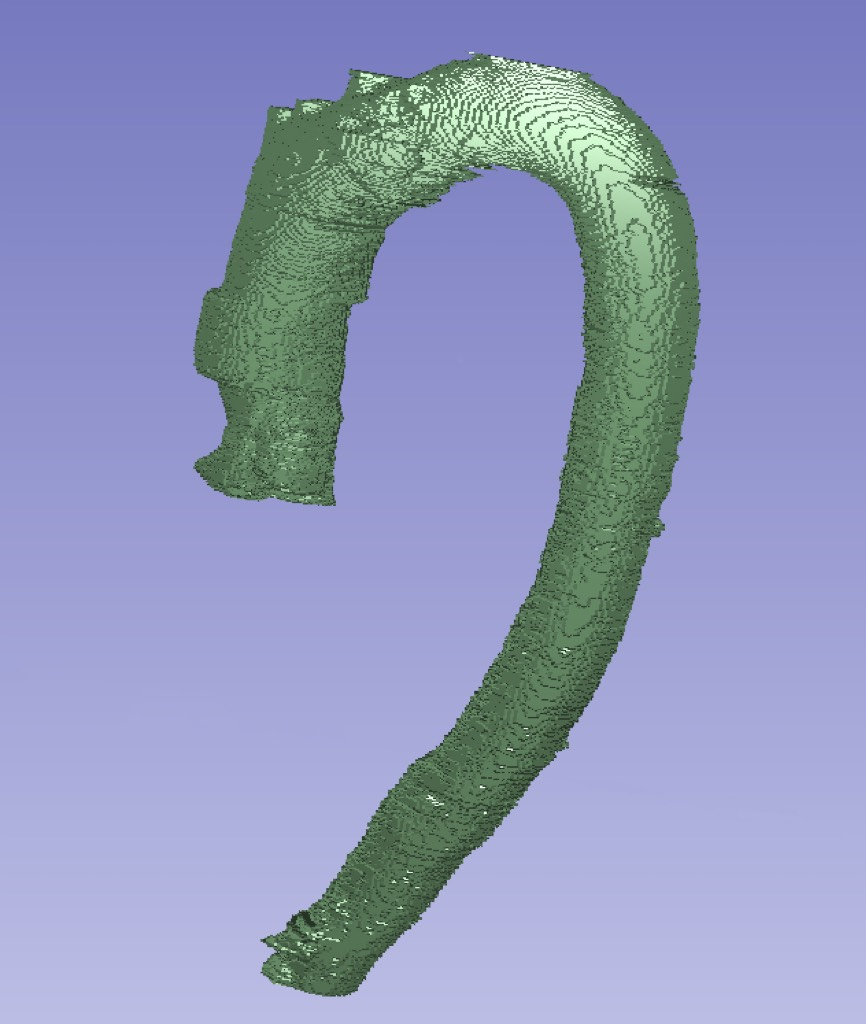
\includegraphics[width=0.5\textwidth]{figures/AGR/segmentation_result.jpg}
    \caption[Segmentation Result]{Segmentation Result}
    \label{fig_sr}
\end{figure}

\section{3D Slicer Extension Development}
The project has started from a simple segmentation program build in Jupyter Notebook \cite{Kluyver2016jupyter}, inherited from a previous developer (Kailin Chu). With this program, the user needs to investigate the chest CT scans using another software (like 3D Slicer or ITK-Snap), to get the necessary input readings, such as coordinates and size to crop (the coordinates of the yellow dots shown in Figure~\ref{fig_aorta_seed}).

\begin{figure}[H]
    \centering
    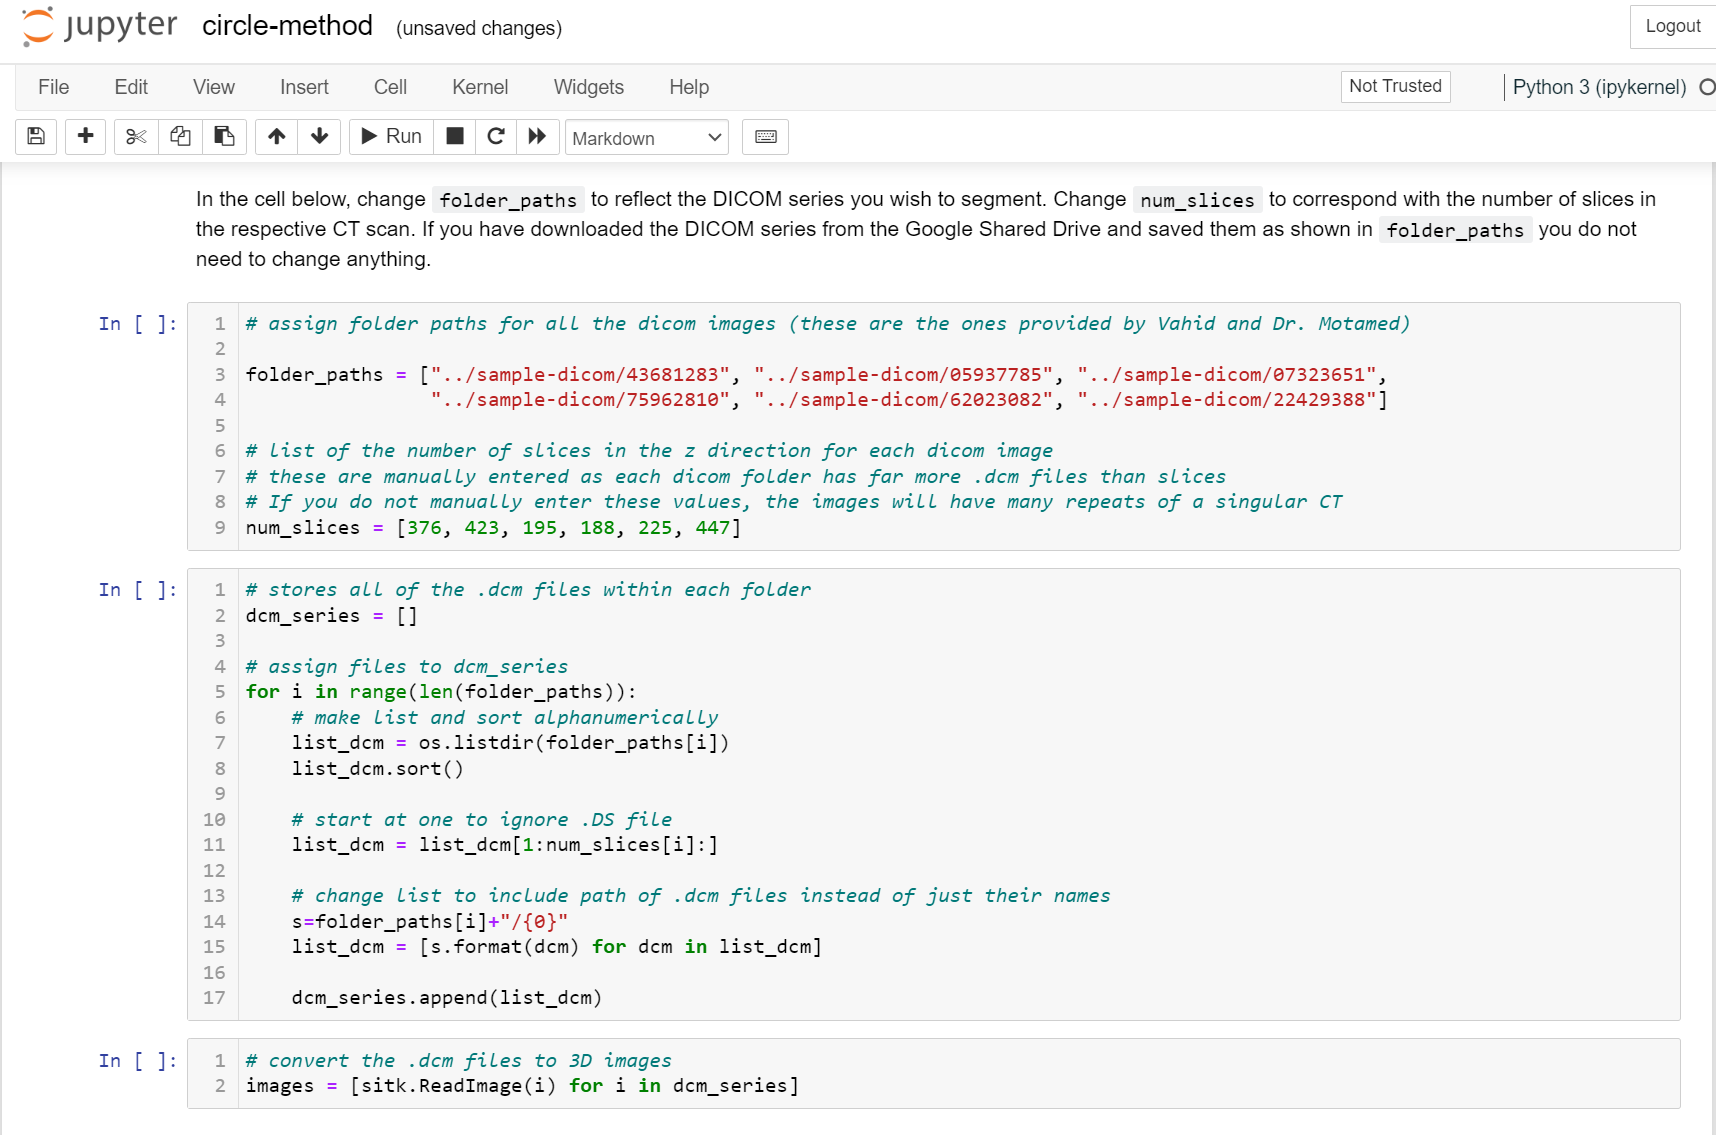
\includegraphics[width=\textwidth]{figures/AGR/jupyter_research.png}
    \caption[Jupyter Notebook Research]{Jupyter Notebook Researched by Kailin Chu}
    \label{fig_jnr}
\end{figure}

Originally, the parameters entered by the users, and many other values were hard-coded in the Jupyter Notebook. To improve the usability of the \progname{} (reduce the amount of time for user inputs and execution), we implemented an extension module on 3D Slicer. 

3D Slicer is an open-sourced medical image processing software for research. 3D Slicer provides useful modules such as Crop Volume module and Volume Rendering module that easily crop any volume. 3D Slicer is highly modular with Python scripting to control the extension module sequence, and QT designer to generate Graphical User Interfaces.

3D Slicer supports modularization with an extension. An extension can compose multiple modules, where each module is dedicated to solve a sub-problem.

\subsection{3D Slicer's data structure}

3D Slicer's Data Structure can be divided into two categories. The Node data structure stores large data such as DICOM, with a Volume Node, Volume rendering Region of Interest Node, and Label Map Volume Node. The parameters are stored as strings from the UI component of the module. Every data stored in 3D Slicer can be accessed by the 3D Slicer's Widget Class and Logic Class for further processing. 

3D Slicer stores all the above data in a scene object, which is also referred to as a MRMLscene file, on the higher level data format. 3D Slicer can load any MRMLscene file, this allows the user to retrieve all the data nodes and parameters. In addition, 3D Slicer has a special input module for the DICOM database that allows users to store DICOM metadata.

\subsection{3D Slicer's scripted module}

Every ScriptLoadableModule in 3D Slicer have a Widget Class and a Logic Class. The Widget Class is used to initialize the extension module's UI component, and the parameters tied to the UI component. The module's Logic Class is used to perform the processing of the data. In the Logic Class, we initialize an AortaGeomRecon Segmenter object with the attributes set to the parameters reading from the UI component, which are inputs by the user. After completing the segmentation with the Segmenter object, we convert the SimpleITK image object to a volume node corresponding in 3D Slicer, which allow the user to visualize the segmentation result. 

\subsection{AortaGeomReconDisplayModule}

In this section, we demonstrate the implementation details of the 3D Slicer plugin AGR. We first demonstrate the module's Graphical User Interface, then discuss the module's logic and workflow.

\subsubsection{Graphical User Interface}\label{GUI}

\begin{figure}[H]
    \centering
    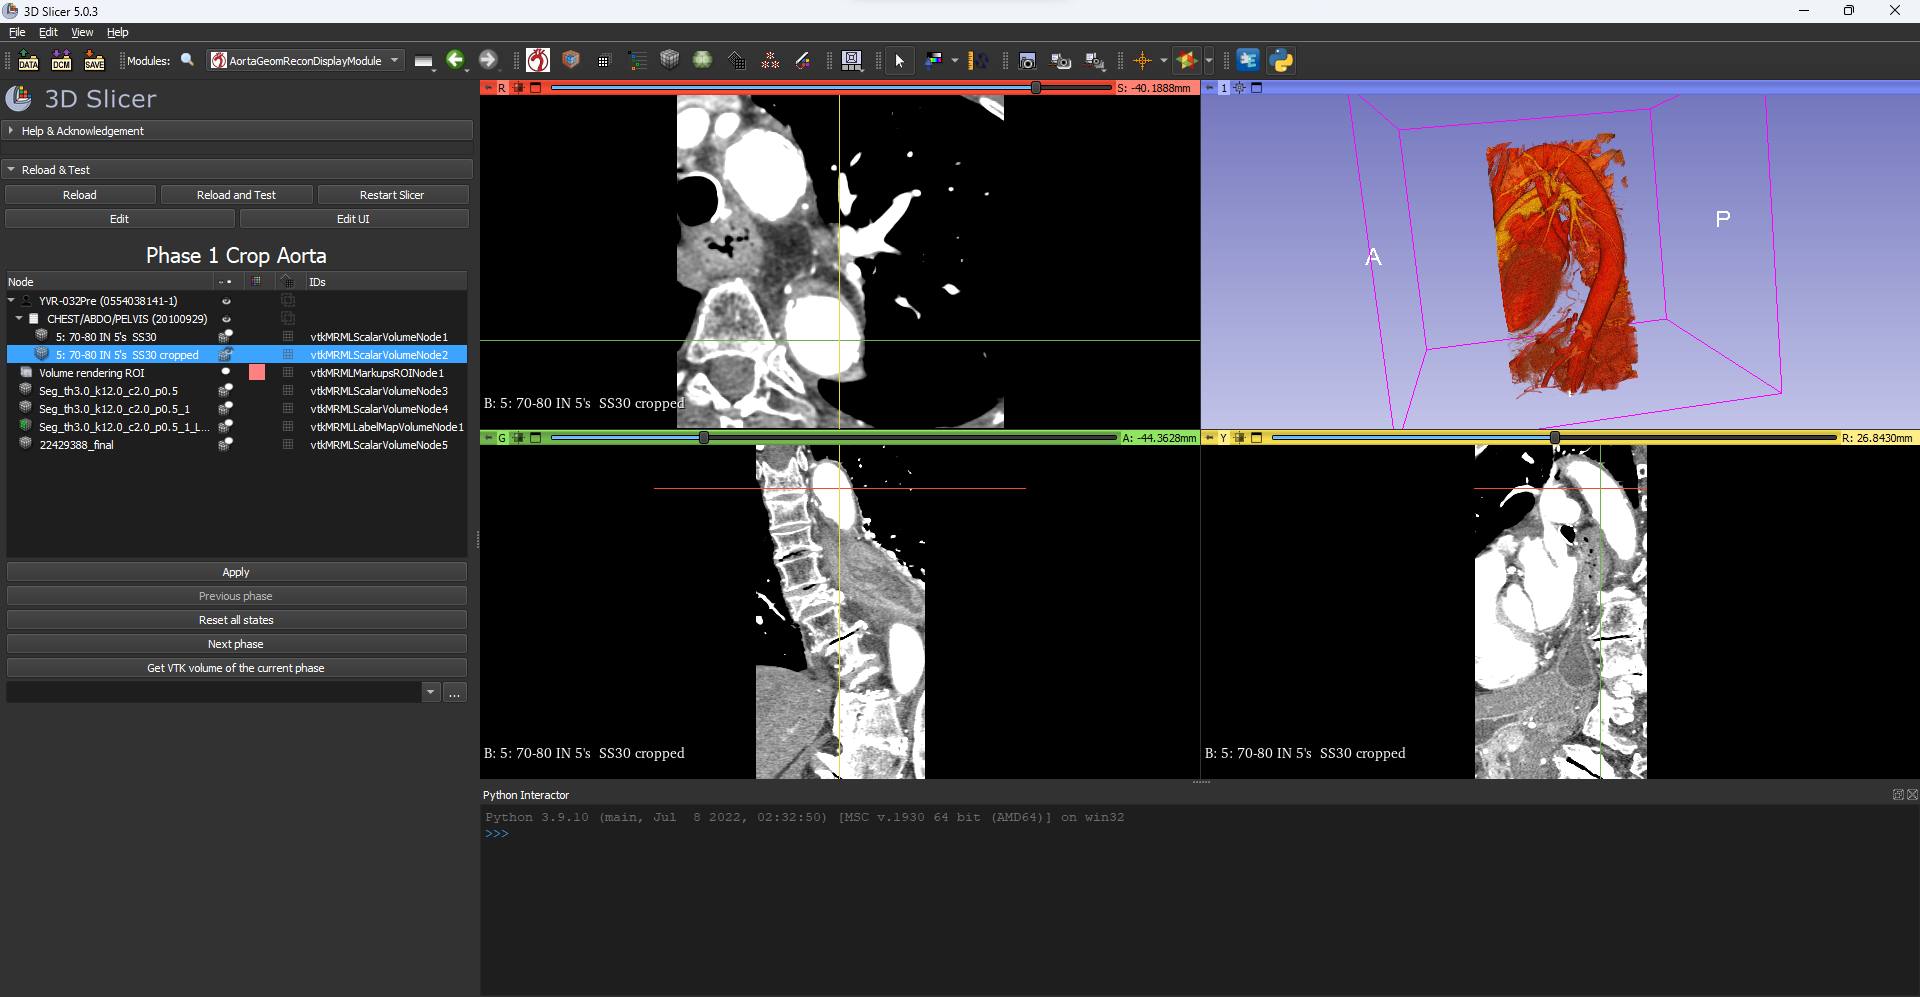
\includegraphics[width=\textwidth]{figures/AGR/Slicer_UI.png}
    \caption[3D Slicer UI]{3D Slicer UI}
    \label{fig_slicer_ui}
\end{figure}

3D Slicer separate the UI into two parts. From Figure~\ref{fig_slicer_ui}, we can see that the four windows on the right side of the UI are used to visualize a volume. The left side shows the SubjectHierarchyTreeView where the module stores many data nodes. The first node is the DICOM patient data with the chest CT scans stored as a volume, and the cropped volume as generated with Crop Volume Module. There is a Volume rendering Region of Interest (ROI) node and several ScalarVolumeNode, which are the generated segmentation volume with different parameters.

The left side is the module UI. This part is designed and implemented differently based on the requirements of the modules. The Figure~\ref{fig_module_ui} shows the module UI that the AGR implements, where each parameter is stored to be passed to the algorithm class.

\begin{figure}[H]
    \centering
    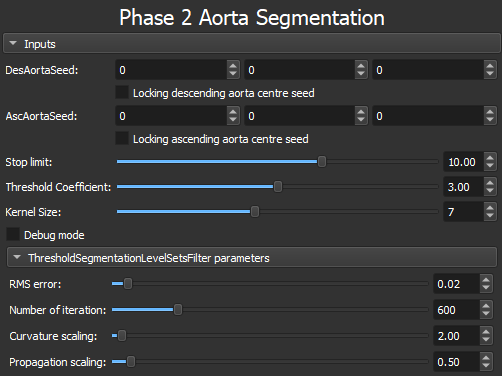
\includegraphics[width=0.7\textwidth]{figures/AGR/Module_UI.png}
    \caption[AortaGeomRecon Module UI]{AortaGeomRecon Module UI}
    \label{fig_module_ui}
\end{figure}


\subsubsection{Module's Workflow} \label{module_workflow}
When the user first starts 3D Slicer and clicks on the AGR module, the warning message and tips shown in Figure~\ref{fig_agr_warning} appear in the module's UI. The user must clicks on the confirm button below to proceed into the next steps. This warning message is a part of the evidence for the assurance case, as explained in the next chapter.

\begin{figure}[H]
    \centering
    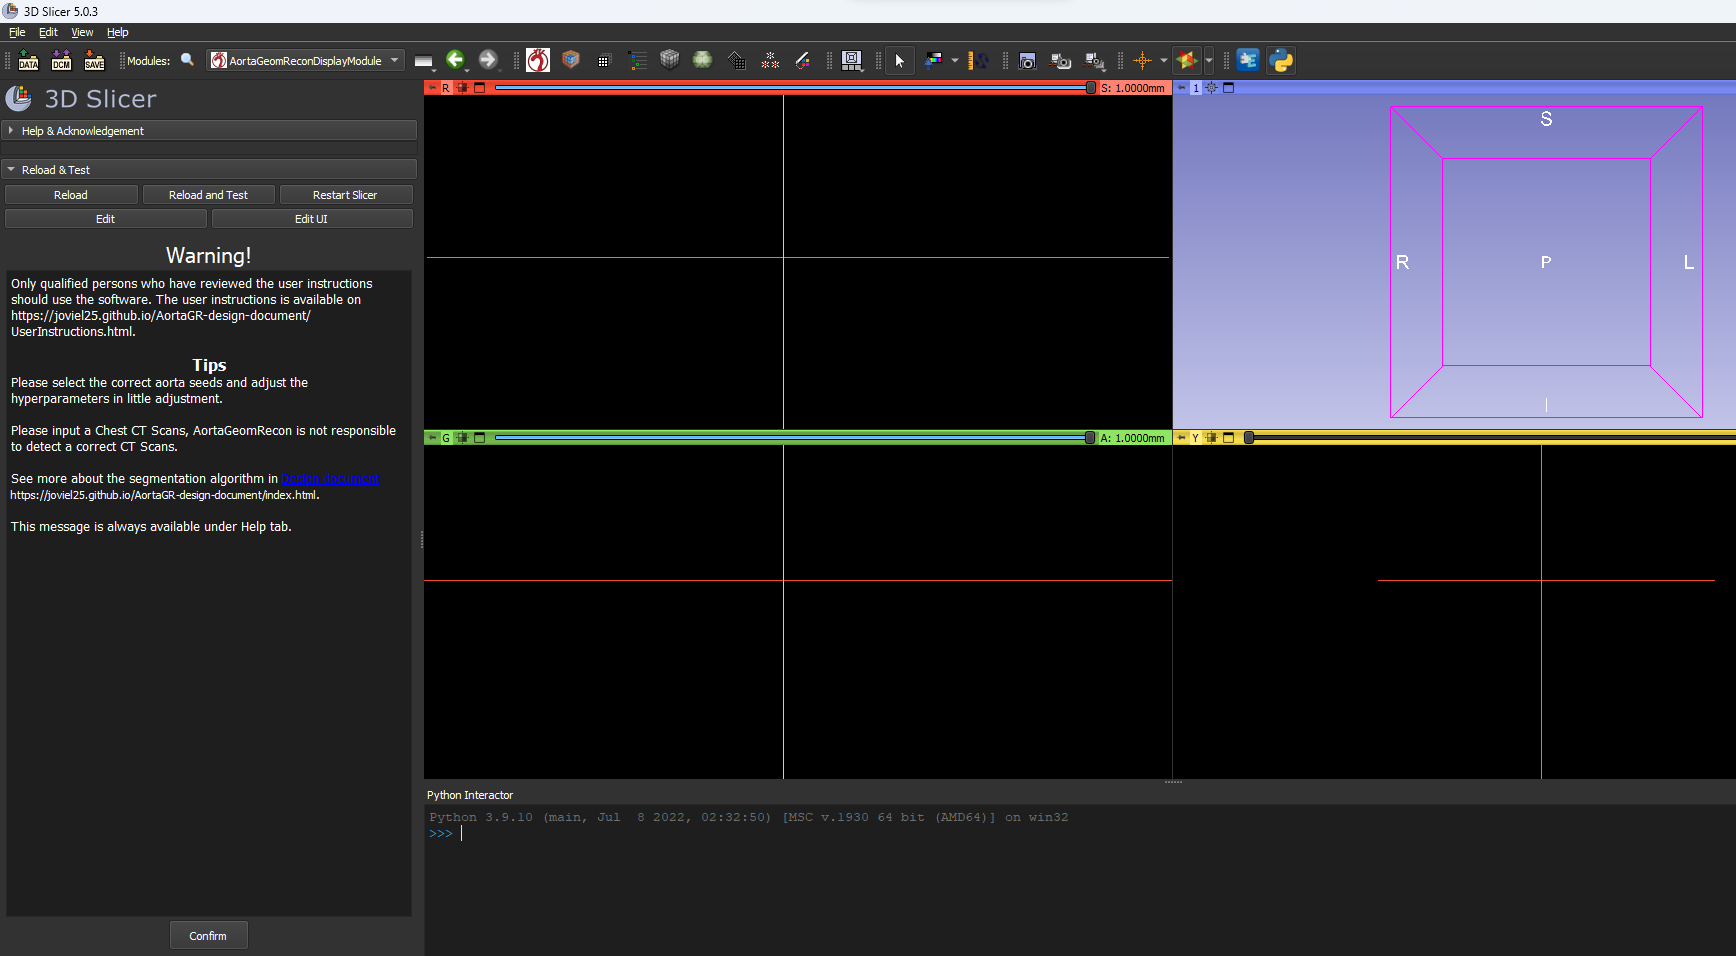
\includegraphics[width=\textwidth]{figures/AGR/AGR_warning.png}
    \caption[AortaGeomRecon Warning message]{AortaGeomRecon Warning message}
    \label{fig_agr_warning}
\end{figure}

In the next step, assuming that the user has already read a DICOM image of the patient's chest, the user is asked to generate a cropped volume using the 3D Slicer's Volume Rendering module and the Crop Volume module. In this phase, the module UI displays only a SubjectHierarchyTreeView where the large data node are shown in this view. After generating a cropped volume, the apply button is enabled and the user can proceed to the next step.

In phase 2 aorta segmentation, the user is asked to input the parameters to perform the segmentation. The module UI is same as Figure~\ref{fig_module_ui}. The necessary inputs are the two aorta seeds. Without any value for these two inputs, the module will not allow the user to generate a segmentation result. One of the advantages of using 3D Slicer is the interactive UI that supports reading coordinates on the volume interactively. On the right side of the Figure~\ref{fig_slicer_ui}, we see a crossed intersection pointing to parts of the aorta, this intersection point allows the developer to read the coordinates. Moreover, we were able to automatically pick up the coordinates in real-time in the coordinate widget. As the user moving the intersection, we get the coordinate readings. Figure~\ref{fig_module_ui} also demonstrates that the user can lock a seed, so the program stops picking up newest coordinate from the intersection point.
